\section{Exact finite construction}
\label{app:dm-conditional}
Fix \(D\) finite categorical fields and a nonempty admitted corpus with positive integer source weights.
For a supported prefix \(u\), let \(n(u)\) be the total weight of all tuples beginning with \(u\).
Its normalised suffix law is \(p(v\mid u)=n(uv)/n(u)\).
At each cut identify exactly those prefixes with equal suffix laws.
Equality gives the same next-symbol probabilities.
Conditioning on a supported next symbol then gives equal remaining laws, so the successor state is well defined.
Unsupported symbols have probability zero and contribute no branch.

Along a supported tuple, successive conditionals telescope:
\begin{equation}
 \begin{aligned}
 \prod_{g=0}^{D-1}t_g(a_g,x_g)
 &=\prod_{g=0}^{D-1}\frac{n(x_0\cdots x_g)}{n(x_0\cdots x_{g-1})}\\
 &=\frac{n(x)}{W}.
 \end{aligned}
\end{equation}
The empty-prefix count is \(W\).
Multiplication by \(\prod_gf_g(x_g)\) and summation over paths proves Eq.~\eqref{eq:querymass}.
Summing paths from the terminal proves Eq.~\eqref{eq:adjoint}.
A suffix of identity tests has conditional probability one.
For an event test \(f\) contained in a conditioning test \(h\), the normalised answer is \(Z(f)/Z(h)\) only when \(Z(h)>0\).
The two calculations must use the same empirical law and source revision selection.

The fixed field order is part of the representation.
The quotient may approach the full prefix trie for a poorly structured law.
Neither conditional sharing nor a citation to ordered decision graphs implies a small representation for arbitrary data.
Likewise, retaining source witnesses does not make witness enumeration free.
The source-to-tuple incidence and unmerged prefix counts are additional stored information, not silently included in the quotient's byte count.

\subsection{Integer messages}
\label{app:dm-integer}
Probability messages can be evaluated without fractions in the validated Boolean setting.
For each continuation node \(a\), write its positive suffix probabilities as primitive integer weights \(c_i/T_a\), where the \(c_i\) have greatest common divisor one and sum to \(T_a\).
Define the scaled message
\begin{equation}
 \widetilde m_a=T_a m_a .
\end{equation}
For a Boolean product test, \(\widetilde m_a\) is the integer sum of the primitive weights that pass the remaining tests.
Thus \(0\leq\widetilde m_a\leq T_a\).
At the terminal, \(T_{\rm term}=1\) and \(\widetilde m_{\rm term}=1\).
For the suffix law \((3/4,1/4)\), the primitive total is four.
The test selecting the first category has scaled message three and probability message \(3/4\).
This conversion is what the integer implementation preserves.

Suppose edge \(a\to b\) has reduced probability \(r/\ell\), with \(\gcd(r,\ell)=1\), and the child's suffix probabilities are \(c_i/T_b\).
The branch weights are \(rc_i/(\ell T_b)\).
Their least common denominator is
\begin{equation}
 \frac{\ell T_b}{\gcd(r,T_b)}.
 \label{eq:dm-branchdenom}
\end{equation}
Taking the least common multiple over supported branches gives the parent's primitive total \(T_a\).
The integer edge multiplier is
\begin{equation}
 J_{a,x}=\frac{T_a\,t_g(a,x)}{T_{\delta_g(a,x)}} ,
\end{equation}
and
\begin{equation}
 \widetilde m_a=\sum_xJ_{a,x}f_g(x)\widetilde m_{\delta_g(a,x)} .
 \label{eq:dm-integer}
\end{equation}
The empirical root count is \((W/T_{\rm root})\widetilde m_{\rm root}\).
We use \(D\) for the number of fields, \(\ell\) for a rational denominator, \(s\) for a source and \(a\) for a continuation node.
Divisibility and overflow checks precede integer execution.
Ordinary float32 or float64 contraction of rational transitions is a separate numerical path.
Signed, non-Boolean or unbounded effects are not automatically integer queries.

\section{Witnessed source revisions}
\label{app:dm-updates}
The initial immutable files contain these exact ASCII assertions, each followed by a newline:
\begin{quote}\small
Group 00 contains 4 records with A=0 and B=0.\\
Group 01 contains 1 records with A=0 and B=1.\\
Group 10 contains 1 records with A=1 and B=0.\\
Group 11 contains 4 records with A=1 and B=1.
\end{quote}
The factor order is \(A,B\), with cardinalities \(2,2\).
Each group denotes a distinct batch.
The parser requires its group identity to match the logical source identity.
For \texttt{d01-r1}, the retained assertion is the complete second line, its weight is one and its tuple is \((A,B)=(0,1)\).
The parser checks the immutable bytes against their supplied hash, the full literal grammar, positive integer weight and group-to-source identity.
It records the whole assertion span and the count's subspan.
A malformed assertion or mismatched group is refused, and the engine checks the total-weight bound before mutation.
Replay of the same revision reads and hashes the bytes but neither reparses nor adds the weight again.
These are implemented admission rules for this literal fixture.
They do not decide whether two natural-language reports describe the same event.
That identity policy, and support for every admitted field, remain required inputs outside this grammar.

The correction changes source 00's count from four to three in a new immutable revision.
Both assertion spans are \([0,45)\), and the count span is \([18,19)\).
The added source says exactly
\lq\lq Group 02 contains 1 records with A=0 and B=1.\rq\rq\
The grammar's \lq\lq 1 records\rq\rq\ is preserved.
Batch 02 is distinct from batch 01, even though they contribute to the same tuple.
Retraction of 01 removes only its old contribution.
Active source selection, content hashes, assertion locations and contributions are retained together.

\begin{table}[h]
\caption{Complete admitted state sequence.
Counts are ordered \((n_{00},n_{01},n_{10},n_{11})\).
The replay is an event attempt but does not create a new count state.}
\label{tab:dm-edits}
\begin{ruledtabular}
\begin{tabular}{lcc}
Operation & Counts & \(P(B=0\mid A=0)\)\\
\hline
Initial & \((4,1,1,4)\)&\(4/5\)\\
Correct 00 & \((3,1,1,4)\)&\(3/4\)\\
Add 02 & \((3,2,1,4)\)&\(3/5\)\\
Retract 01 & \((3,1,1,4)\)&\(3/4\)\\
Replay corrected 00 & \((3,1,1,4)\)&\(3/4\)\\
Change 10 to 12 & \((3,1,12,4)\)&\(3/4\)\\
Change 10 to 8 & \((3,1,8,4)\)&\(3/4\)\\
Retract 00 & \((0,1,8,4)\)&\(0\)\\
Retract 02 & \((0,0,8,4)\)&undefined\\
\end{tabular}
\end{ruledtabular}
\end{table}

The update engine stores source incidence, tuple totals and an unmerged prefix trie.
An occurrence is an aggregate raw prefix keyed by its ordered field values, not a source-labelled copy.
The source catalogue separately retains one incidence entry per active revision.
For example, after correcting 00 and adding 02, the exact active records include
\begin{quote}\small
\texttt{d01-r1}: Group 01 contains 1 records with A=0 and B=1.\\
\texttt{d02-r1}: Group 02 contains 1 records with A=0 and B=1.
\end{quote}
Each has weight one, tuple \((0,1)\), assertion span \([0,45)\) and count span \([18,19)\).
They have distinct source hashes and revisions.
The incidence list for \((0,1)\) contains both entries, while \texttt{counts[(0,1)]} is two and the single raw path is \(()\to(0)\to(0,1)\).
Its leaf count two is normalised to the same empty-suffix law as every positive terminal.
The \(A=0\) prefix has aggregate counts \((3,2)\), total five and canonical conditional law \((3/5,2/5)\).
Removing \texttt{d01-r1} retracts weight one from that tuple and removes that source entry only.
The raw leaf survives with count one through \texttt{d02-r1}.
Its parent now has counts \((3,1)\) and binds to law \((3/4,1/4)\).
The previous canonical law is not edited.
This is the distinction that source-labelled-prefix wording would obscure.
A canonical signature contains reduced rational outgoing probabilities and successor-signature identities in a fixed category order.
Interning an already present signature reuses its immutable state.
Reference counts track active occurrences of those states.
This allows counts \((3,1)\) and \((12,4)\) to share a law, then split when the latter becomes \((8,4)\).

A query binding is keyed by raw prefix occurrence and query suffix and points to the canonical state used for that evaluation.
A canonical cache entry is keyed by immutable state identity and the remaining factor sequence.
An edit invalidates affected occurrence bindings.
It need not delete a correct message attached to an unchanged immutable signature.
If an earlier signature recurs, that message can be reused.
For a correction at \((0,0)\), the changed occurrence path contains root, \(A=0\) and its \(B=0\) leaf.
For a change at \((0,1)\), it contains the other leaf.
Root probabilities may change even when a child's conditional suffix is unchanged.

Each field test is one of \((1,1),(1,0),(0,1),(0,0)\), giving sixteen product queries.
At all nine recorded states, a source catalogue maintained independently of the engine follows the declared event protocol.
One oracle reparses every active file with an independent token parser and rebuilds aggregate conditional laws.
Another decomposition directly enumerates weighted rows with integer and rational arithmetic.
Their values agree with the incremental backwards messages and forward channels in all 144 query-state checks.
Source identities, witness spans, tuple multisets, active references and immediate old-root immutability are also checked.
These are related exact checks, not 144 independent statistical experiments.

Two further attempts are refused before mutation: a total beyond the signed 64-bit-compatible bound and a mismatched group identity.
The fixture exercises eight admitted event attempts, two refusals and at most five logical documents.
It tests replay, merge, split and zero conditioning support.
It does not test arbitrary conflicting bytes under one revision, tuple-changing replacements or a completely empty corpus.
The source grammar and input policy are part of this finite result.

For fixed order \(D\) and bounded category count \(c\), a changed tuple touches at most \(D+1\) raw prefixes.
Copying child slots and hashing local signatures costs \(O(Dc)\) slot work, in addition to changed-source processing, dictionary operations and rational bit complexity.
For \(Q\) fixed queries, at most \(O(QD)\) ancestor binding checks arise on that path.
Actual message recalculation is charged to the affected dependency cone.
Many changed tuples or a changed field order can affect many paths.
The implementation does not establish a uniform sublinear update bound.

Early nontrivial fixture edits invalidate 24 active bindings, copy four child slots and examine four transition slots.
The count of 24 comes from query-specific bindings on the affected ancestors, not 24 different source documents.
Retained engine history grows from 30,062 to 67,052 bytes because old signatures and messages remain immutable.
Replay still reads and hashes the source, but requires neither reparsing nor path copying.
The complete traced CPU fixture reports 68.90 ms pre-output CPU time and 69.03 ms wall time, peak RSS 43,732,992 bytes and traced peak memory 815,161 bytes.
Tracing excludes some interpreter/native allocation, whereas RSS includes the process.
Limits are 60 s CPU and 128 MiB virtual address space.
Reconstruction, direct evaluation and the residual harness are verification costs.
These measurements are not isolated update-latency or scaling-speedup estimates.

\section{Selective channels}
\label{app:dm-channel}
The extra question here is representational: can classical selection be embedded in an operation that remains positive when the memory is part of a larger system?
A density matrix \(\rho\) is positive semidefinite, with trace equal to its total mass.
Diagonal entries are populations in a chosen basis.
Off-diagonal entries, called coherences, distinguish an amplitude superposition from a classical mixture.
An auxiliary system is any additional register whose correlations we retain rather than discard.
Complete positivity requires positivity on the combined system for every such register.
This is stronger than checking nonnegative classical populations.

Let \(\mathcal H_g\) be the vector space with orthonormal basis indexed by continuation states at cut \(g\).
For each supported pair \((a,x)\), Eq.~\eqref{eq:kraus} maps \(\mathcal H_g\) to \(\mathcal H_{g+1}\).
There is no independent output index to sum without a successor restriction.
The map
\begin{equation}
 \Phi_g^f(\rho)=\sum_{a,x}K_{g,a,x}\rho K_{g,a,x}^{\dagger}
\end{equation}
has a Kraus representation, so it remains positive when tensored with any identity map.
The dagger denotes conjugate transpose.
Its completeness sum is
\begin{equation}
 \begin{aligned}
 \sum_{a,x}K_{g,a,x}^{\dagger}K_{g,a,x}
 &=\sum_a q_g(a)|a\rangle\langle a|\leq I_{\mathcal H_g},\\
 q_g(a)&=\sum_xt_g(a,x)f_g(x).
 \end{aligned}
\end{equation}
Thus it is trace-nonincreasing for \(0\leq f_g\leq1\), and trace-preserving when the step is unfiltered.
On diagonal populations it reproduces \(M_g^f\) and removes input coherences.
Normalising by a positive selected trace is nonlinear.
Signed or greater-than-one effects need not define a trace-nonincreasing instrument.

\subsection{Why square-root amplitudes require a separate gauge}
The classical extension above must not be confused with amplitude tensors
\begin{equation}
 V_g^x[b,a]=\sqrt{t_g(a,x)}\,\mathbf1[b=\delta_g(a,x)] .
\end{equation}
The alternative representation stores square roots of probabilities as amplitudes, so squared amplitude gives outcome probability.
The \emph{future amplitude environment} is the vector of amplitudes for all remaining symbol sequences.
Its Gram matrix contains their pairwise inner products.
Different continuation labels can describe nonorthogonal future amplitude vectors.
This overlap is why ordinary orthonormal-state completeness is the wrong test for the raw \(V^x\).
Gu et al.\ use nonorthogonal predictive quantum states to reduce memory in stochastic simulators~\cite{Gu2012e2bbbd}.
Our gauge makes a finite amplitude realisation consistent with its own inner product.
It does not establish that our representation attains their memory advantage.
For the suffix laws \((.8,.2)\) and \((.2,.8)\),
\begin{equation}
 V^0=(\sqrt{.8},\sqrt{.2}),\quad
 V^1=(\sqrt{.2},\sqrt{.8}),
\end{equation}
and
\begin{equation}
 \sum_x(V^x)^\dagger V^x=
 \begin{pmatrix}1&.8\\.8&1\end{pmatrix},
\end{equation}
rather than the identity.
This Gram matrix describes overlap of amplitude environments, not failure of the classical conditional law.

Write \(H_g\) for the actual suffix-amplitude Gram matrix, reserving \(Z(f)\) for query mass.
With \(H_D=1\),
\begin{equation}
 H_g=\sum_x(V_g^x)^\dagger H_{g+1}V_g^x .
\end{equation}
On its support, define
\begin{equation}
 B_g^x=H_{g+1}^{1/2}V_g^xH_g^{-1/2}.
\end{equation}
Then \(\sum_x(B_g^x)^\dagger B_g^x\) is the support projector.
No inverse is introduced on a null direction.
Positivity of the Gram recursion implies
\(H_{g+1}^{1/2}V_g^xv=0\) whenever \(v\in\ker H_g\).

For a compatible root amplitude \(r\), prepare \(H_0^{1/2}r\) with \(r^\dagger H_0r=1\), and use the same Gram environments at every cut and the terminal \(H_D=1\).
The factors \(H_g^{1/2}\) and \(H_g^{-1/2}\) cancel on supported paths.
In the one-root empirical construction, \(r=1\) and its path amplitudes are \(\sqrt{p(x)}\).
The gauge therefore preserves the joint outcome law.
Multiplication by \(\sqrt{f_g(x)}\) supplies a supported selective instrument.
This is a supplementary amplitude realisation, not machinery used by the text selector.

The stored float64 fixtures check the off-diagonal overlap .8, nonsingular gauge, joint law \((.4,.1,.1,.4)\) and a singular support projector at tolerance \(10^{-12}\).
The recorded completeness defect is \(2.22\times10^{-16}\), joint-law defect \(1.67\times10^{-16}\) and singular-support defect zero.
They are finite numerical checks accompanying the algebra, not a physical-time interpretation.

\section{Optional retained dynamics}
\label{app:dm-memory}
The query problem starts with a fixed empirical law and asks for a selected expectation.
An additional modelling problem is to predict observables under a specified evolution.
Its input is a finite column Markov generator \(G\), meaning nonnegative off-diagonal rates and zero column sums, and an evolving probability vector \(\rho(t)\) satisfying \(\dot\rho=G\rho\).
We assume a fixed positive stationary distribution \(\pi\) and detailed balance
\(G_{ij}\pi_j=G_{ji}\pi_i\).
For a source graph, \(G\) could be a declared reversible diffusion with specified edge rates.
It is not inferred physical kinetics merely because sources are linked.

Set \(W_\pi=\diag(\pi)\) and
\begin{equation}
 L=W_\pi^{-1/2}GW_\pi^{1/2},\qquad
 y=W_\pi^{-1/2}(\rho-\pi).
\end{equation}
Detailed balance makes \(L\) symmetric and nonpositive.
A chosen \(n\times r\) isometry \(U\), \(U^{\mathsf T}U=I_r\), selects the \(r\) retained directions from \(n\) source states.
The retained fluctuation is \(z=U^{\mathsf T}y\), and the omitted fluctuation is
\(\eta=\Pi_\perp y\), where \(\Pi_\perp=I-UU^{\mathsf T}\).
Thus \(y=Uz+\eta\).
These signed fluctuations are not density matrices or positive source masses.

Define the retained generator \(A=U^{\mathsf T}LU\), coupling \(B=U^{\mathsf T}L\Pi_\perp\) and omitted generator
\(L_\perp=\Pi_\perp L\Pi_\perp\) on \(\Ran\Pi_\perp\).
Then
\begin{equation}
 \dot z=Az+B\eta,\qquad
 \dot\eta=B^{\mathsf T}z+L_\perp\eta .
\end{equation}
Solving the second equation by variation of constants and substituting gives
\begin{align}
 \dot z(t)&=Az(t)+B e^{tL_\perp}\eta(0)\nonumber\\
 &\quad+\int_0^t B e^{(t-u)L_\perp}B^{\mathsf T}z(u)\,du .
 \label{eq:dm-memory}
\end{align}
The kernel records excursions into omitted directions and their return to retained observables.
The initial forcing carries omitted preparation.
Both vanish if \(B=0\).
This is the finite reversible version of projection and orthogonal propagation in Mori's Sections 2--3~\cite{mori}.
Time \(t\) is the declared evolution parameter, not the query cut \(g\).
No continuous numerical run is claimed for the source-update fixture.

The saved four-state calculation fixes a symmetric nearest-neighbour generator
\begin{equation}
G=\begin{pmatrix}
-1&1&0&0\\
1&-1.3&.3&0\\
0&.3&-2.3&2\\
0&0&2&-2
\end{pmatrix},\qquad
\pi=\tfrac14(1,1,1,1)^{\mathsf T}.
\end{equation}
Rates share an arbitrary inverse-time unit, and \(L=G\) for this uniform reference.
Choose the observables first: to predict masses in groups \(\{1,2\}\) and \(\{3,4\}\), retain
\begin{equation}
U_2=\frac1{\sqrt2}
\begin{pmatrix}1&0\\1&0\\0&1\\0&1\end{pmatrix}.
\end{equation}
The omitted directions are imbalances inside the groups.
Putting more mass on state 2 than state 1 changes the flux across the \(2\leftrightarrow3\) edge even if their group total is unchanged.
The term \(B^{\mathsf T}z\) creates such an imbalance, \(e^{tL_\perp}\) propagates it, and \(B\) returns its effect to the group masses.
Dropping the convolution keeps \(Az\) but loses this delayed contribution.

The saved rank-three choice appends \((1,-1,0,0)^{\mathsf T}/\sqrt2\) to \(U_2\), retaining one internal imbalance explicitly.
Rank four retains all coordinates.
Figure~\ref{fig:dm-four-state} shows the resulting kernels and the error from replacing \(U^{\mathsf T}e^{tL}U\) by \(e^{tA}\), for preparation \(y(0)=Uz(0)\).
The recorded coupling norms are \(0.300\), \(0.260\) and zero.
Choosing \(U\) from an intended observable, then adding internal directions that reduce its omitted component or dynamical coupling, gives the projection a purpose.
A small rank alone does not guarantee closure.
These are existing controlled evolution data, not an evolution run of the source-update fixture.
\begin{figure*}[t]
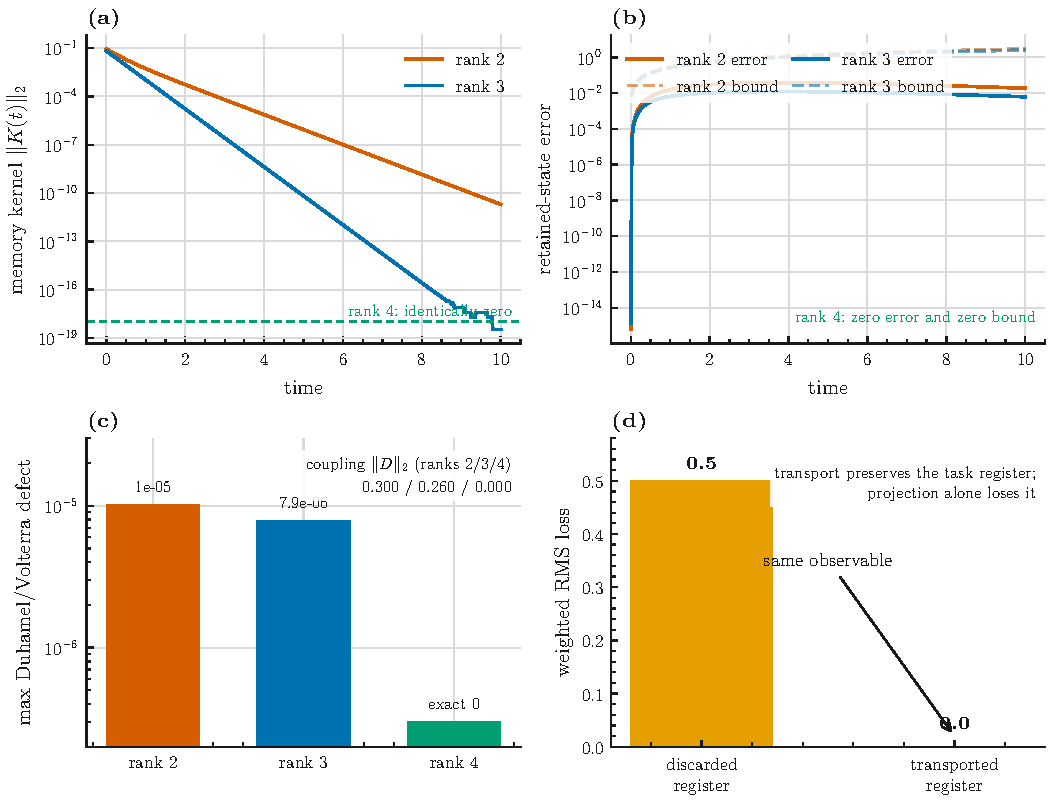
\includegraphics[width=.9\textwidth]{../../../extension/figures/controlled_effective_dynamics_v1.pdf}
\caption{Saved four-state illustration with the generator and retained spaces specified above.
(a) Kernel norm for ranks two and three, with rank four identically zero.
(b) Operator error from omitting memory, bounded by \(t\|B\|_2\).
(c) Residual from trapezoidal evaluation of the exact Volterra equation on the saved grid \(t=0,.025,\ldots,10\).
This quadrature defect is not a model error.
The figure's coupling \(D\) denotes the present \(B\), not the number of categorical fields.
(d) For observable \(f=(0,1,0,1)\), discarding within-group coordinates loses a reference-weighted RMS component \(1/2\), while carrying all internal coordinates gives zero loss.
The example explains which information must accompany group mass when that observable is needed.}
\label{fig:dm-four-state}
\end{figure*}

Positive coarse masses require their own preparation.
Let \(C\) be a \(k\times n\) partition aggregator, with \(C_{\alpha i}=1\) when source state \(i\) belongs to coarse group \(\alpha\).
Let \(\pi_c=C\pi\), assume all groups have positive mass, and define
\begin{equation}
 R=W_\pi C^{\mathsf T}\diag(\pi_c)^{-1},\qquad CR=I_k .
\end{equation}
The column of \(R\) is the reference distribution conditional on that group.
For the preparation \(\rho(0)=R\rho_c(0)\), the coarse propagator
\(T_c(t)=Ce^{tG}R\) is stochastic.
It need not satisfy a semigroup law:
\begin{equation}
 T_c(t+u)-T_c(t)T_c(u)
   =Ce^{tG}(I-RC)e^{uG}R .
\end{equation}
A general preparation \(R\rho_c(0)+\eta_{\rm raw}\), with \(C\eta_{\rm raw}=0\), adds \(Ce^{tG}\eta_{\rm raw}\).
Exact lumpability \(CG=G_cC\) is sufficient for closure.

The partition is a special retained subspace.
Specifically,
\(U_C=W_\pi^{1/2}C^{\mathsf T}\diag(\pi_c)^{-1/2}\)
is an isometry.
A general \(U\) may retain extra signed within-group directions.
For a source test \(f\), write \(a=W_\pi^{1/2}f\).
The reconstructed expectation from \(z\) is
\begin{equation}
 \widehat{\langle f\rangle}
     =f^{\mathsf T}\pi+a^{\mathsf T}Uz ,
\end{equation}
whereas the actual expectation is \(f^{\mathsf T}\rho\).
Their error is
\(a^{\mathsf T}(I-UU^{\mathsf T})y\), giving
\begin{equation}
 \left|\langle f\rangle_\rho-\widehat{\langle f\rangle}\right|
 \leq\|(I-UU^{\mathsf T})a\|
              \sqrt{\chi^2(\rho\Vert\pi)} .
\end{equation}
Here \(\chi^2(\rho\Vert\pi)=\sum_i(\rho_i-\pi_i)^2/\pi_i\).
For \(\rho=\pi(\cdot\mid E)\) with \(\pi(E)=b>0\), this factor is \(\sqrt{b^{-1}-1}\).
A residual norm bounds missing expectation, not the omitted original passage.

If a second isometry \(U_2\) acts on all coordinates retained by \(U_1\), the composite is \(U_1U_2\).
Passing only positive coarse masses while discarding the retained internal coordinates does not implement that composition.
The inherited reference and reconstruction maps must also be passed.
This specifies the composition without introducing an undefined hierarchy of grades or decoders.
It is an optional mathematical result, not an implemented language-pipeline stage.

\section{Structured query protocol}
\label{app:dm-timings}
The primary law enumerates all \(2^{D-1}\) assignments of the first \(D-1\) bits, sets the last bit to even parity and uses unit integer weights.
Dimensions are \(D=13,\ldots,19\).
All tuples are distinct.
Query batches contain \(1,32,256,1024\) positive Boolean product tests.
They fix \(r=0,1,2,4,8,D-1,D\) coordinates, with duplicates removed.
Locations are prefix, suffix or evenly spread when applicable, plus none for \(r=0\) and all for \(r=D\).
Values are taken deterministically from supported witness rows.
Thus the tests have positive empirical mass.
For \(r<D-1\), support fraction is \(2^{-r}\), and for \(r=D-1,D\) it is \(1/N\).

The packed direct comparator evaluates bit masks without materialising a query-by-row matrix.
The weighted-unique comparator first aggregates identical codes and weights.
On the primary law both have \(N\) unique rows.
The exact continuation comparator uses the validated primitive integer representation with a fused width capacity of 128.
That number is an implementation capacity, not a theorem bounding continuation width.
Preflight refuses excess width or memory before preparation.

Two warmups precede eleven samples per served method and shape.
Kernel times use CUDA events.
Full-API wall intervals synchronise the device and include the query API boundary.
The plotted per-regime value is its median full-API time.
The main figure aggregates all nontrivial parity regimes at each size and batch count: the line is their median and the shading their minimum-to-maximum range.
The range describes different queries and locations, not a confidence interval.
Support diagnostics collapse batch count, leaving 112 distinct dimension/fixed-count/location regimes.

The saved matrix records a device-memory total of 3,953,721,344 bytes and explicit resident memory/headroom.
A device model identifier is not present in that matrix.
The timings therefore remain specific to its recorded 4 GB CUDA environment.
A hardware-normalised performance comparison is not established here.
First-use compilation, construction and the source/witness bank are outside the warm query boundary and are reported separately.

\begin{figure*}[t]
\centering
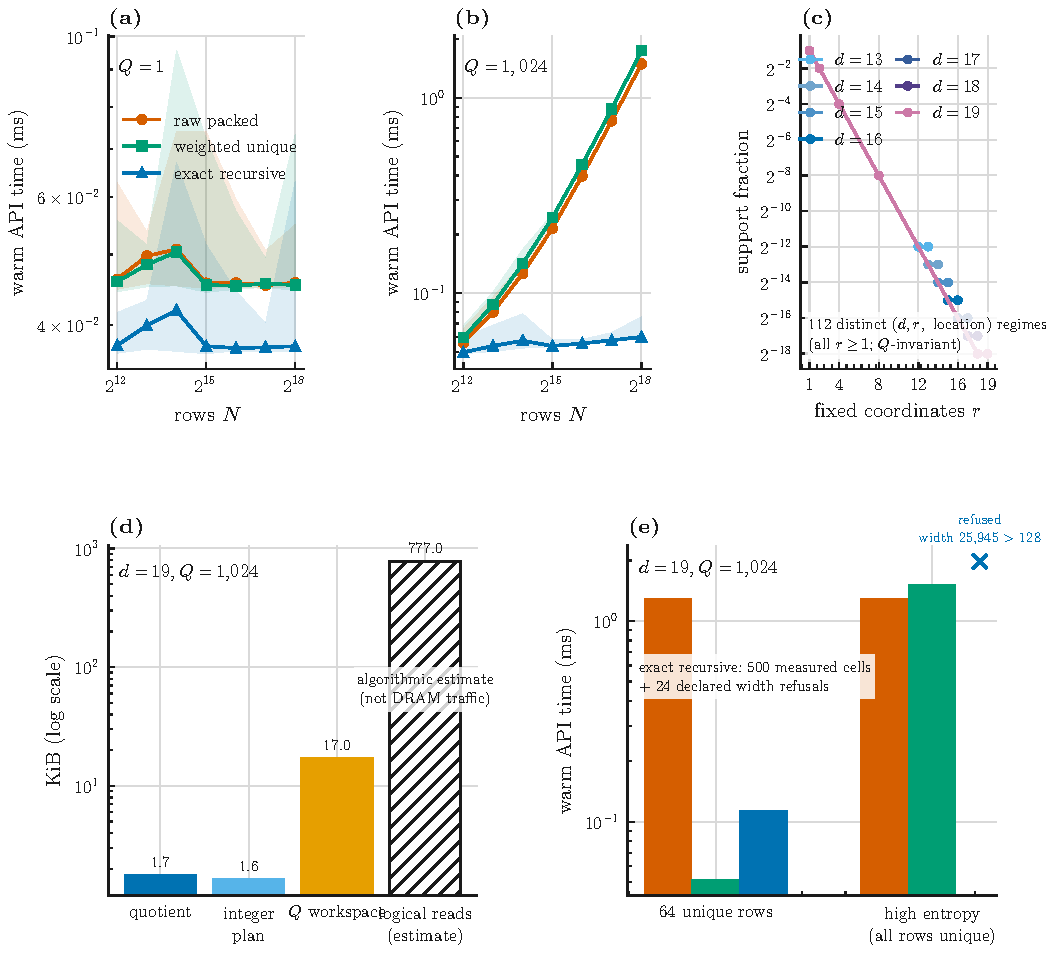
\includegraphics[width=\textwidth,viewport=0 246 504 458,clip]{../../../extension/figures/query_locality_completed_v1.pdf}\\[1ex]
\begin{minipage}[t]{.49\textwidth}\vspace{0pt}\centering
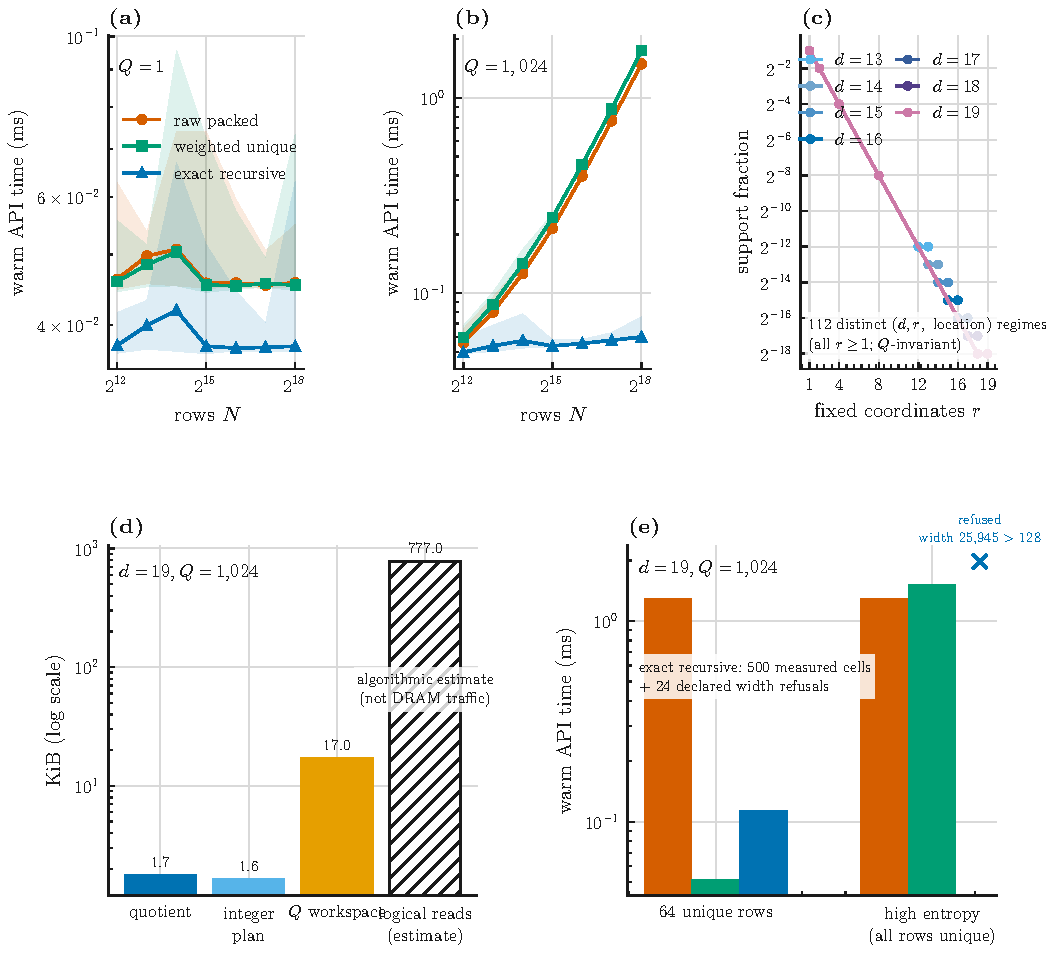
\includegraphics[width=\linewidth,viewport=0 27 247 216,clip]{../../../extension/figures/query_locality_completed_v1.pdf}\\[-.5ex]
{\scriptsize\hspace*{.17\linewidth}\begin{tabular}{cccc}
quotient & integer & query & logical\\
 & plan & workspace & reads (est.)
\end{tabular}}
\end{minipage}\hfill
\begin{minipage}[t]{.49\textwidth}\vspace{0pt}\centering
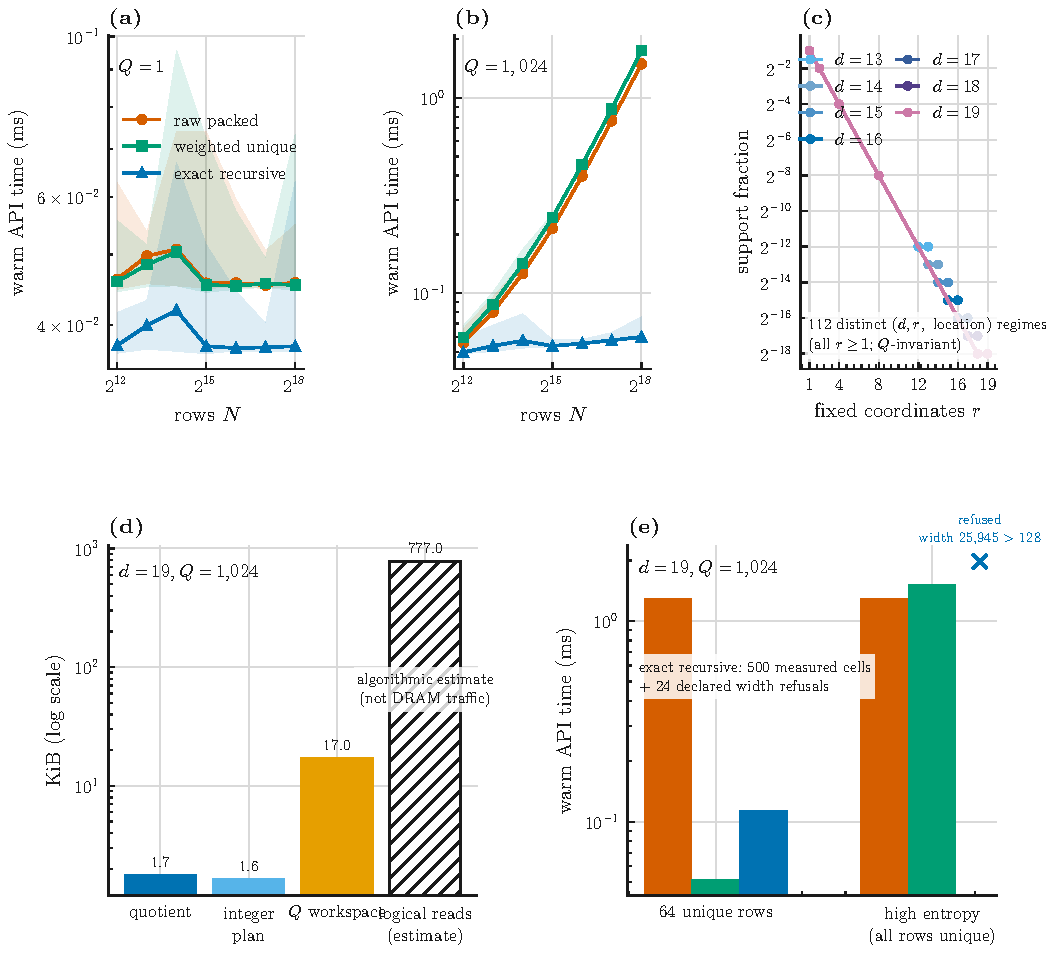
\includegraphics[width=\linewidth,viewport=258 0 504 216,clip]{../../../extension/figures/query_locality_completed_v1.pdf}\\
{\scriptsize Orange: raw packed. Green: weighted unique.\\Blue: exact continuation (cross: width refusal).}
\end{minipage}
\caption{Complete structured-query diagnostic.
(a,b) The parity latency panels used in the main paper.
(c) Query support fraction as the number \(r\) of fixed coordinates changes, for \(D=13,\ldots,19\).
(d) For \(D=19,Q=1024\), quotient storage, integer plan, query workspace and estimated logical reads are different costs.
The last bar is an algorithmic byte-load estimate, not measured DRAM traffic.
(e) Separate control laws, not the parity family: a repeated 64-world support favours weighted direct evaluation, while high-entropy unique support exceeds the continuation kernel's width capacity.
All five original panels are retained as vector crops, with resource labels reset below (d) and an explicit method legend beside (e).
\lq\lq Exact recursive\rq\rq\ in the saved plot means exact continuation evaluation by the integer messages above.
Orange circles denote raw packed scanning, green squares weighted-unique scanning and blue triangles continuation evaluation in (a,b).
The same method colours apply to (e), whose blue cross is a refusal, not a timing.}
\label{fig:dm-all-timings}
\end{figure*}

The secondary laws use a seeded unique half-support of all bit strings, or 64 deterministic unique worlds repeated to the same row count.
They use \(D=13,16,19\), fixed counts four and \(D-1\), and evenly spread locations.
There are 524 recorded cells in all.
Exact continuation executes 500 and agrees with direct integer evaluation.
The remaining 24 are declared width refusals on high-entropy supports.
At \(D=19\), that control has width 25,945 rather than two.
The repeated 64-world support favours the weighted direct method.

At the largest parity size, the weighted-unique control takes \(1739.6\,\mu\mathrm{s}\) per 1024-query batch.
The continuation and integer add-on together use about 3.4 kB, excluding sources, witnesses and query workspace.
Extra construction costs about 55 ms.
Warm precompiled crossover is about 6500 individual single-query calls, or roughly 29,000--41,000 \emph{individual} queries when submitted in batches of 1024.
The latter is of order tens of batch invocations, not tens of thousands of batch invocations.
First-use compilation adds a separate cost.
These are regime-specific amortisation accounts, not a universal speedup.

For an overflow-safe sorting build, comparison and prefix-slot work is bounded by
\(O(DN\log N+\sum_gP_gc_g)\), with \(P_g\) unmerged prefixes.
The compact quotient may be much smaller than that input.
The GPU implementation uses immutable snapshots followed by full construction.
The CPU revision fixture described above is separate.
Its success cannot be combined with these GPU timings into a measured incremental-GPU speedup.

\section{Text methods}
\label{app:dm-text}
The news and FRAMES cohorts were originally drawn by a deterministic stratified rule.
Within each dataset stratum, questions not in the recorded prior-exposure set were sorted by SHA-256 of \texttt{salt|dataset|qid}, using salt \texttt{relational-frontend|draw-order|v1}, and the first quota entries selected.
News uses 43 each of comparison, temporal, inference and null questions, giving 172.
Null questions ask for information the supplied news collection does not establish.
FRAMES uses 38 each of Multiple constraints, Numerical reasoning, Post processing, Tabular reasoning and Temporal reasoning, giving 190.
For a question with several reasoning labels, the loader's rarest-label stratum supplies its allocation.
The originally excluded exposure sets contain 112 news and two FRAMES questions.
Subsequent development inspected these drawn questions and used their failures to develop delivery and reader instructions.
Their initial draw status does not make the present follow-ups untouched confirmation.
The fit/check halves alternate sorted question IDs within each stratum and are preserved as development labels, not restored independence.

LongMem here means the cleaned LongMemEval-S task~\cite{longmem}, not the unrelated LongMem model.
The completed comparison uses the earlier September final-48 manifest, disjoint from the later 188-question draw and the separate 24-question development set.
Its quotas are seven each of single-session user recall, assistant recall, user preference, multi-session integration, temporal reasoning and knowledge update, plus six abstentions.
The manifest records selection salt \texttt{skein-longmemeval-s-cleaned-v1}.
These 48 questions have also been examined during development.
Their dialogue histories supply the observations, while the question date anchors requested elapsed times.

The finite fixture tests update correctness for admitted counts.
The parity study tests structure-dependent query cost.
The news comparison tests evidence assembly under two stated reading operations.
FRAMES tests source delivery and a missing-needs continuation under a fixed answer rubric.
The shared-index LongMem comparison tests the delivered outcomes of its actual index and packing configuration.
It is not a test of a distinct compressed conditional algorithm.
No score is pooled across these purposes or cohorts.

The common news representation contains 609 articles.
Each article is the title followed by its body.
Two-sentence windows have stride one sentence.
Their vector representation is a 384-component BGE-small-en-v1.5 embedding of the text prefixed by title, outlet and publication date.
The imported fp16 encoder produces the stored half-precision rows, which are dotted in float32 for scoring.
Question and facet vectors use its query role.
Cosine compares unit-normalised vectors in this same space.
A document identity names the article, whereas an outlet label can name many articles.
A window retains its character interval in its article.
The matcher can therefore separate article presence from delivery of the required passage.

The deterministic outlet grammar recognises stored outlet names, a leading-\lq the\rq\ alias and the prefix before a vertical bar where present.
It resolves overlapping mentions in favour of the earlier longest match.
Question clauses split at \lq while\rq\ or \lq whereas\rq.
A date following an outlet mention binds locally, otherwise a leading date can be shared.
With no outlet mention, the initial facet is the whole question with no outlet binding.
This is a finite metadata grammar, not a universal natural-language compiler.

The slot compiler uses the same admitted metadata vocabulary as the source index.
Publication-role dates admit the exact day.
Event or unresolved-role dates admit the declared window from that day through six days later.
A month with a year but no day conditions the stored month label.
Missing time or outlet conditions leave that axis unrestricted.
Unknown labels pass unrestricted axes but fail a known-value constraint.
Support membership is the conjunction of allowed metadata labels on the article's retained tuple.
A recognised outlet or fine-day condition with no supported article gives an empty set, not an invented replacement source.
A month mask is formed only for labels present in the stored coarse vocabulary.
If no month label is recognised, that axis stays unrestricted.
Entity, mechanism and polarity are not hard conditions in the compared news route.

Requirements for table reading are produced by the question compiler, not by a model asked for the answer.
It keeps the question's need text for each recognised outlet/date side and its bound slots.
Where a temporal question names several windows, it emits the dated requirements separately.
The requirement compiler returns an ordered obligation list with IDs, need text, source/date/entity slots and cardinality, plus an operator descriptor \(\{\mathrm{kind},\mathrm{over}\}\) and internal frame parameters.
For news, \texttt{comparison\_query} selects \texttt{compare}.
A \texttt{temporal\_query} selects \texttt{change} when it asks about changed or consistent accounts, or lacks ordering words, and otherwise \texttt{order}.
The change frame records whether \lq yes\rq\ means changed or unchanged, while the order frame records before/after and yes/no form.
Inference and null questions both select \texttt{bridge}.
Thus routing does not reveal a null question's reference abstention.
No gold answer or reference evidence enters compilation.

For the Sporting News question below, the temporal-change rule yields \texttt, \texttt{over=[o1,o2]}, with \lq yes\rq\ meaning changed.
The obligations retain the 4 October ticket-report side and 7 October playoff-report side, each bound to Sporting News and its day.
Their metadata supports are the article sets listed below.
The descriptor says which reports the requested operation needs.
In the reported \texttt{table2} condition it does \emph{not} execute a typed change adjudicator or a numerical event comparison.
The reader receives the obligation needs and bound slots, fills one passage-support row per obligation and writes the answer.
All three retrieval methods receive those same requirements.
Typed witness operators and later growth protocols are separate implementations, not additional stages inferred from these scores.

\subsection{One retained source-to-context trace}
The recorded question is:
\begin{quote}\small
Between the Sporting News report on Inter Miami's season ticket prices following Lionel Messi's arrival published on October 4, 2023, and the Sporting News report on Inter Miami's exclusion from the MLS playoffs published on October 7, 2023, was there a change in the team's postseason prospects as reported by the news source?
\end{quote}
Its two outlet/day supports are Sporting News on 4 October and Sporting News on 7 October.
The former includes article \(d203\), \emph{Inter Miami season tickets: Lionel Messi demand causes 2024 prices soar to most expensive in world}, published at 22:12:56 UTC, and \(d41\), \emph{Chicago Fire vs Inter Miami live score, result, updates, highlights from Lionel Messi in MLS match}, at 23:33:00 UTC.
The latter includes \(d88\), \emph{Inter Miami vs FC Cincinnati live score, result, updates, highlights with Lionel Messi's MLS playoffs on line}, published 7 October at 21:30:00 UTC.
These identifiers distinguish articles, not outlets.

The first retained 2000-token facet-conditioned context uses 1989 tokens and has three original article blocks plus an explicitly derived support table.
The support table lists source identities and dates from retained tuples and is marked as derived, not a passage.
The article blocks merge selected spans in original order, with ellipses at gaps.
The ticket-price block states:
\begin{quote}\small
The pricing structure for 2024 represents an enormous increase over the 2023 costs.
\end{quote}
The earlier match block says Messi \lq\lq did not arrive with the team\rq\rq.
The later match block states:
\begin{quote}\small
Eventually, Alvaro Barreal's 78th-minute goal ended any hope that Inter Miami had to complete a stunning playoff charge, and the defeat coupled with CF Montreal's big 4-1 victory over Portland means Inter Miami are officially out of the postseason running.
\end{quote}
The requested comparison needs an earlier postseason assessment as well as later elimination.
The named ticket article and a match-availability statement do not automatically supply that earlier assessment.
The stored diagnostic marks one of three required facts absent from this context.
We present this as a delivery trace, not a newly judged answer or a fabricated successful reconstruction.

The table-reading prompt supplies requirement IDs, need text, bound outlet and bound date.
For each requirement the reader must return the IDs of passages that state it, or an empty list, and at most 25 words recording what they state, or \lq not stated\rq.
It then writes the answer and cited evidence IDs.
This is an explicit reader operation, not a truth value attached by the selector.
Answer-form rules instead require short alternatives, yes/no answers or an insufficient-information response without the table.
The same rule and schema are applied within each comparison.

\subsection{Assembling evidence}
For every route, cosine scores are combined with \(0.5\) times a BM25 keyword score normalised by its maximum over the scored set.
BM25 uses \(k_1=1.2,b=.75\).
The facet-conditioned route ranks within each exact support, retains up to 400 candidates per facet and merges the lists round-robin with duplicate removal.
A short derived support table is admitted only when its standalone token cost is at most one quarter of the evidence budget.
The diversity-ranked route takes 200 whole-corpus candidates and uses MMR relevance coefficient .7.
The local recursive-summary route searches its 1747 stored summaries together with the shared labelled window layer, without MMR.
RAPTOR's distinction between traversal and collapsed retrieval is methodological context~\cite{raptor}.
This local comparator uses the collapsed approach with adapted leaves and packing.
Its summaries are existing abstractive cluster summaries, not empirical conditional states.
The stored hierarchy was built recursively from embedded 100-token leaves using UMAP reduction and Gaussian-mixture memberships, then summarising each cluster and embedding its summary for the next level.
The local implementation uses GPU clustering with declared fixed-seed/update deviations from public RAPTOR.
The summary adapter requests faithful preservation of names, dates, relations and qualifications, caps each summary at 100 tokens and stores it as a distinct parent node.
The reported comparison reuses those summary texts and their BGE vectors, substituting the common labelled-window leaf layer.
It neither regenerates summaries for this test nor makes the generated text an original source witness.

Packing considers ranked spans in order.
It groups them by article, extends them to sentence boundaries, merges touching spans and presents each article's spans in original order.
Articles are ordered by their best admitted piece.
Gaps are marked, not filled with generated text.
Summary nodes remain separate fixed blocks.
The 2000-token allowance counts the canonical JSON serialisation with \texttt{cl100k\_base}, including labels and metadata.
The reader is Claude Sonnet 5.5 at low effort.
The endpoint is normalised exact match from the preserved scorer.
Needed-fact coverage is diagnostic: a reference fact counts only when a mapped occurrence lies inside the union of delivered original spans of its article.
Reference annotations are used for that diagnostic and scoring, not to choose candidate passages.

The banked extraction path stores a proposed statement even when none of its support quotations survives location checking, marking it \texttt{no\_witness}.
Quote matching normalises whitespace and quote characters only, then requires a substring of that input unit.
Unmatched quotations are dropped, not converted into support.
The downstream tuple assembler retains statement status and witness flags beside categorical fields and sparse piece-to-entity, outlet, day/page and document incidence.
It does not thereby certify semantic support for those fields or turn them into the weighted \((A,B)\) fixture.
The compared news route uses hard source/date support and passage ranking, not these statement fields as an entailment gate.

The finite query construction and this text route share explicit source conditions and retained evidence identities.
The news context stage reuses exact supported article sets and ranks original windows within them.
It does not perform a source-edit experiment, propagate the continuous memory kernel, or assign the exact weighted-record demonstration's correctness to language extraction.
The derived support table is distinguished from original text throughout.
The text results measure the delivered evidence and reader response for the stated configuration.

\section{Additional text outcomes}
\label{app:dm-extra-text}
Figure~\ref{fig:dm-news-rules} preserves the common answer-form condition.
It gives 152, 152 and 148 exact matches, with facet-conditioned discordances \(6\)--\(6\) against diversity ranking and \(9\)--\(5\) against local summaries.
The requirement-table condition in the main paper instead gives \(153/145/147\), with \(9\)--\(1\) and \(7\)--\(1\).
The reader operation therefore changes the observed comparison.
Fact-delivery counts remain \(234/211/205\).
The original within-type alternating split has 88 fit and 84 check questions.
Requirement-table exact-match counts are fit \(78/75/77\) and check \(75/70/70\), in facet-conditioned/diversity/local-summary order.
Answer-form rules give fit \(76/77/75\) and check \(76/75/73\).
These original strata describe the same examined cohort and retain their labels without a held-out claim.
They do not isolate the causal effect of the requirement table or establish selector superiority on fresh questions.
\begin{figure*}[t]
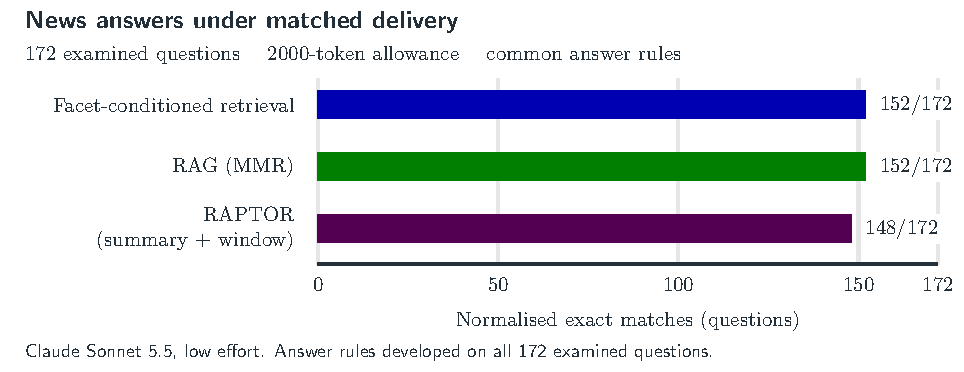
\includegraphics[width=.94\textwidth]{figures/generated/mip_news_matched.pdf}
\caption{Matched-news figure, showing the \emph{answer-form rules} condition.
It is not the requirement-table row in the main paper.
The evidence allowance, labelled windows and local summary adaptation are held fixed within this condition.
\lq\lq RAPTOR\rq\rq\ in this saved figure denotes the adapted local recursive-summary comparator, not a fresh public-system reproduction.
The tie between facet-conditioned and diversity-ranked retrieval is important to the interpretation of the main result.}
\label{fig:dm-news-rules}
\end{figure*}

\begin{table*}[t]
\caption{Additional news method configurations, kept separate from the common-window comparison.
The first row is a different 48-question news cohort, not LongMem, balanced at 12 questions per news type.
The other rows reuse the fixed 100-token-leaf contexts with distinct reader settings.
No score is pooled across rows.}
\begin{ruledtabular}
\begin{tabular}{lrrrr}
Configuration & Questions & Source-conditioned & Flat retrieval & Local summaries\\
\hline
100-token passages, Sol reader &48&40&39&35\\
100-token fixed contexts, Sonnet 5.5 low &172&133&125&118\\
100-token fixed contexts, Sol 5.6 low &172&140&132&130\\
\end{tabular}
\end{ruledtabular}
\end{table*}
In the fixed-context configuration, flat retrieval uses cosine top 40 on 100-token leaves, MMR .7, at most 20 objects and first-fit packing.
The local RAPTOR index has 14,359 leaves and 1747 summaries, takes its cosine top 20 and uses the same local first-fit packing limit.
The allowance is 2000 \texttt{cl100k\_base} tokens.
The stored tree and vectors are reused without a fresh build.
The 48-question configuration also has a flat metadata control with 40 correct answers and byte-identical contexts to the source-conditioned route.
The first row supplies an end-to-end configuration observation on a different draw.
The two 172-question rows hold each method's stored 100-token contexts fixed while changing the reader.
They show sensitivity to reading configuration, not a fresh retrieval gain, a controlled comparison against the common-window route or an isolated effect of the conditional quotient.

\subsection{FRAMES}
FRAMES evaluates retrieval, factual response and reasoning together~\cite{frames}.
The retained source-conditioned comparison uses no entity-activation narrowing beyond its declared source route.
Its initial candidate head comprises fifty pieces ranked by cosine plus .2 normalised BM25.
The implementation recovers page links by exact registered-title mentions in passage text, not by fetching live hyperlinks.
For the selected \texttt{link:mass} route, scores of the top twenty pieces are accumulated on the pages they name.
The five largest target-page totals contribute their best question-scoring piece, followed by the remaining ranked tail.
This is one recovered title-link hop.
Entity-activation witnesses are off in the reported configuration.
Merged sections combine selected spans from the same source section before delivery.

The initial evidence allowance is 8000 tokens, with an instruction to make the necessary reasoning steps explicit.
A missing fact identified by the reader triggers at most one further retrieval and up to 4000 tokens of new spans.
For the diversity control, pass-one relevance is
\(r+.4h/\max h\), with \(r=\mathrm{cosine}+.2\,\mathrm{BM25}/\max\mathrm{BM25}\) and \(h\) the dense seed score.
MMR's relevance coefficient is separately .7 on 200 candidates.
Pass two ranks a missing-need phrase using \(r(\mathrm{phrase})+.5r(\mathrm{question})\), with its own MMR.
Title binding occurs in the \emph{missing-need pass}, not as an oracle mapping the initial question to answer pages.
The title dictionary is built from registered ingested page titles.
The matcher tokenises the reader's need phrase, starts at capitalised or digit-leading tokens, and tries the longest registered sequence of at most eight tokens.
Its last token must also be capitalised or digit-leading.
Matching itself is case-folded.
For example, a phrase naming \emph{Kermanshah Province} aims at that page only if its tokens match a registered title.
It is not a semantic entity resolver.
For each named page, the source-conditioned route prepends its three highest-scoring pieces under \(r(\mathrm{phrase})+.5r(\mathrm{question})\), then appends the global top-200 phrase ranking.
With no recognised title, that global list is the fallback.
Lists from at most six missing phrases are interleaved and deduplicated.
Already delivered intervals are subtracted, residual pieces shorter than 40 characters are discarded, and merged new spans are packed to 4000 tokens.
The reader sees the old blocks followed by these new blocks.
The diversity control instead applies its own MMR to each phrase list.
Allowances and reading instructions match.

The completed outcomes are 127 versus 126 judged correct and 123 versus 117 lexical-proxy successes on 190 questions.
The judged paired discordances are seven wins and six losses.
The judging agent for these completed follow-ups is Claude Sonnet 5.5 at low effort, using the inherited FRAMES rubric, not the earlier P3 judge's Codex model.
It sees the question, benchmark reference answer and prediction, but not the retrieved passages.
A correct answer must give the same final entity, number, date or alternative as the reference, allowing compatible wording, abbreviations, units and reference-tolerated rounding.
Every required part must be present.
A wrong required part, incompatible value or hedging between alternatives is incorrect.
A refusal is abstained and counts as unsuccessful.
Two batch compositions are judged, with a third decision on disagreement and majority as the final verdict.
This measures reference-answer correctness, not independent verification that cited evidence entails it.

The lexical proxy first accepts normalised exact match.
Otherwise it rejects missing, empty or explicit insufficient-information predictions and any prediction longer than three times the reference's normalised word count.
Normalisation lowercases, removes punctuation and the articles \lq a\rq, \lq an\rq\ and \lq the\rq, then collapses whitespace.
Let \(p\) be the normalised prediction, \(g\) the full reference and \(g_0\) its text before the first full stop or comma, normalised in the same way.
The proxy accepts \(p\subseteq g\), or nonempty \(g_0\) with \(g_0\subseteq p\) or \(p\subseteq g_0\), where \(\subseteq\) here means contiguous substring.
It also accepts token F1 at least .5, using the preserved scorer's token overlap.
This answer-form rule is not semantic correctness.
Figure~\ref{fig:dm-frames} preserves both instead of treating them as the same accuracy measure.
A simpler delivery configuration gives 62/58 judged successes, and an 8k explicit-step configuration before the extra pass gives 106/106.
The large delivery recovery coexists with a small final matched difference.
\begin{figure*}[t]
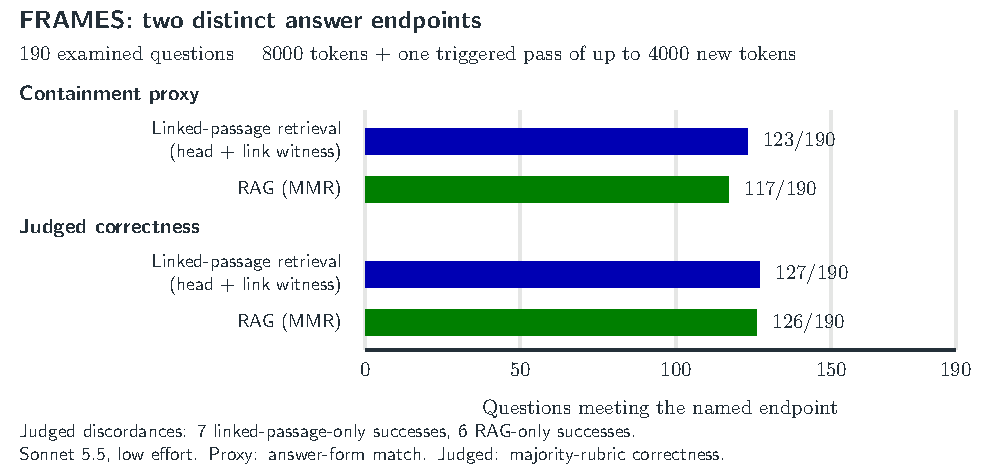
\includegraphics[width=.94\textwidth]{figures/generated/mip_frames_noactivation.pdf}
\caption{FRAMES endpoint comparison.
Lexical-proxy success and judged correctness answer different questions.
Both retrieval routes have the same 8k initial allowance and at most one missing-needs-triggered 4k delivery.
The final judged difference is one answer on 190 questions, not evidence that the methods are equivalent.}
\label{fig:dm-frames}
\end{figure*}

A page in the source bank may omit the required table.
Then page availability is not availability of the needed row.
Other cases deliver relevant facts but require an arithmetic or date operation that the reader fails to complete.
Source availability, located passage support and final correctness identify different points of failure.
Only the completed comparison above is included as an answer outcome.

\subsection{LongMem}
The completed shared-index LongMem comparison retains whole dialogue turns.
Its stored labels \texttt{ours\_keys} (also called relational) and \texttt{dense\_keys} both invoke \texttt{CaseState.dense\_scores("dn",2)}.
There is no distinct compressed conditional reconstruction in this executed arm.
The key \texttt{dn} concatenates the role-labelled raw turn, session date and deterministic normalisations of date mentions and word-form quantities.
Relative expressions are anchored to the turn's session date.
Stored vectors are 384-component BGE-small-en-v1.5 fp16 embeddings, converted to float32 and unit-normalised on loading from the role/text-hashed cache.

For each question-side obligation facet, \texttt{dense\_scores} takes its vector dot product with every turn key.
It then takes a per-turn maximum over the key score, long-turn windows of at most 400 encoder tokens and, with \texttt{views=2}, sentence views of user turns.
Facet-specific stable orders are interleaved round-robin with duplicate removal.
Both arms use these identical facet lists, ties and defaults.
The completed final-48 route has no branch-activation table, no fact ledger and no event-pair operator.
The common packer adds a whole turn when its text tokens plus a twelve-token header allowance fit, skips turns that do not fit, stops below 30 remaining tokens and admits at most 120 turns.
Selected turns are displayed in session-date and within-session order.
Identical question/date/context prompts deliberately share a cached reader response.
Equal predictions here follow equal computation, not an independently measured representation advantage.
The hybrid arm changes the score to .7 times dense plus .3 normalised BM25 before the same facet ordering and packer.

For example, the charity question below asks for two dated events jointly.
The shared-dense score call ranks individual turns, not candidate event pairs.
It has no step that can make both operands obligatory before packing.
This configuration differs from the general exact identities in Eqs.~\eqref{eq:querymass}--\eqref{eq:adjoint} and from the older 32-development-facet transport tests with local vector frames.
Neither is an operation executed by these completed LongMem arms.
The existing figure's \lq\lq Relational retrieval\rq\rq\ label denotes \texttt{ours\_keys}, here a second label for shared-dense execution, not a third reconstruction method.

Correctness includes 48 questions and all six abstentions.
Complete positive evidence uses 42 questions, excluding the six.
Conditional and dense readouts give \(44/48\) and \(45/48\) correct at 4k and 8k, with \(41/42\) positive-evidence coverage at both allowances.
Hybrid gives \(40/48,44/48\) correct and \(33/42,37/42\) positive coverage.
A separate nonempty-annotation endpoint has denominator 44 because two abstention questions also have annotated required turns.
Its preserved counts are \(43/44\) for conditional and dense, and \(35/44,39/44\) for hybrid.
The denominators measure different populations rather than replacing one another.
\begin{figure*}[!htbp]
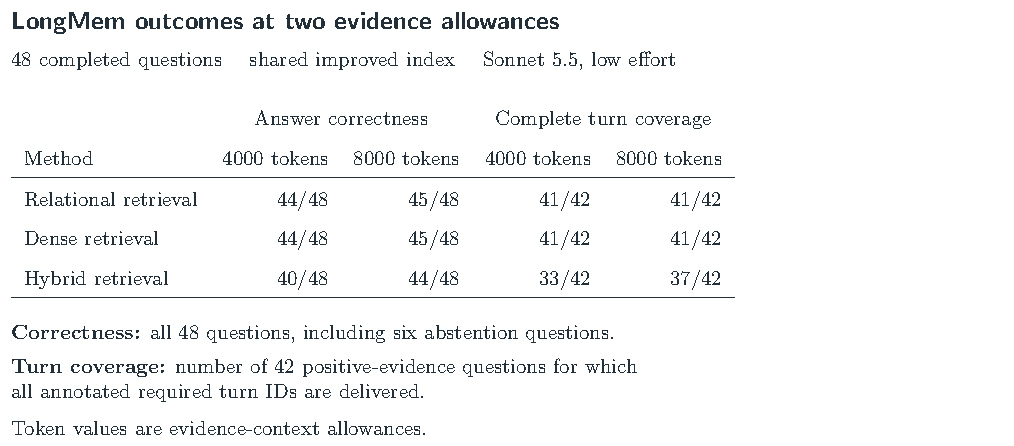
\includegraphics[width=.94\textwidth]{figures/generated/mip_longmem_completed.pdf}
\caption{Completed shared-index LongMem comparison.
Answer correctness includes all 48 questions and six abstentions.
Complete required-turn coverage uses 42 positive-evidence questions.
The saved \lq\lq Relational retrieval\rq\rq\ and dense series are the shared-dense \texttt{ours\_keys} and \texttt{dense\_keys} arms defined above.
They invoke the same score call and packer, not different exact readout implementations.
Evidence-context allowances are 4000 and 8000 tokens.}
\label{fig:dm-longmem}
\end{figure*}

The unresolved positive case asks for elapsed months since two charity events on consecutive days.
Required primary turn ranks are 73, 88, 100, 116 and 134.
The 4k and 8k packs stop after ranks 27 and 54.
The missing primary turns are eligible but not reached before packing stops.
A delivered paraphrase overlaps one event, so primary-ID coverage is not a complete measure of semantic availability.
The decisive pair is not jointly delivered by the executed route.
Hybrid can supply it at 8k but has lower aggregate positive coverage.
This identifies a candidate temporal composition operation to test, not a demonstrated benefit of budget alone.

\par
